\subsubsection{Cross-correlation and convolution of functions}

The convolution of two functions is defined as:
\begin{equation}
h(t)=(p_1\ast p_2)(t)=\int\limits_{-\infty}^{\infty} p_1(t^\prime)p_2(t-t^\prime) \mathrm{d}t^\prime
\end{equation}
\begin{equation}
h(0)=(p_1\ast p_2)(0)=\int\limits_{-\infty}^{\infty} p_1(t^\prime)p_2(-t^\prime) \mathrm{d}t^\prime
\end{equation}
for discrete sequences starting at $i=0$ we have:
\begin{equation}
\boxed{
h(t_i)=(p_1\ast p_2)(t_i)=\sum\limits_{j=0}^{\infty} p_1(t_j)p_2(t_i-t_j)
}
\end{equation}
can be used to obtain the moving average on a data series $\varv_i$  obtained by measuring a variable quantity with a fixed cycle rate $\tau\circ$. The measured sample $\varv_i$ being the value measured and stored at time $t_i=i\tau $.
The window function has the property :
\begin{equation}
\sum\limits_{j=0}^{\infty} w(t_j) = N^\bullet
\end{equation}
The time series will be simply convolved with the normalized window function $w(t_i)\over N^\bullet$
\begin{equation}
\langle \varv \rangle^\bullet_n = \frac{1}{N^\bullet}\sum\limits_{j=0}^{\infty} \varv_{j} w(t_n-t_j)
\end{equation}

one of the most common window function is $\theta_N(t_i)$

\begin{equation}
\theta^\bullet(t_i) = \left\{
\begin{array}{l}
{\displaystyle 1 \qquad \mathrm{ if } \quad \frac{t_i}{\tau^\circ} \in [0,N^\bullet-1]  }\\ \\
{\displaystyle 0 \qquad \mathrm{ if } \quad \frac{t_i}{\tau^\circ} \notin [0,N^\bullet-1]  }
\end{array}
\right.
\end{equation}

\begin{equation}
\langle \varv \rangle^\bullet_n = \frac{1}{N^\bullet}\sum\limits_{j=0}^{\infty} \varv_{j} \theta^\bullet(t_n-t_j)=\frac{1}{N^\bullet}\sum\limits_{j=n-N^\bullet+1}^{n} \varv_{j}=\frac{1}{N^\bullet}\sum\limits_{j=0}^{N^\bullet-1} \varv_{n-j}
\end{equation}



The cross-correlation is given by:
\begin{equation}
h(t)=(p_1\star p_2)(t)=\int\limits_{-\infty}^{\infty} p_1(t^\prime)p_2(t+t^\prime) \mathrm{d}t^\prime
\end{equation}

\begin{equation}
h(0)=(p_1\star p_2)(0)=\int\limits_{-\infty}^{\infty} p_1(t^\prime)p_2(t^\prime) \mathrm{d}t^\prime
\end{equation}

for discrete sequences starting at $i=0$ we have:
\begin{equation}
\boxed{
h(t_i)=(p_1\star p_2)(t_i)=\sum\limits_{j=0}^{\infty} p_1(t_j)p_2(t_i+t_j)
}
\end{equation}


======================


following extract is obtained by using \emph{copy latex} from Maxima (examples intended to help to evaluate the expressions above)
\begin{figure}
	\centerline{
		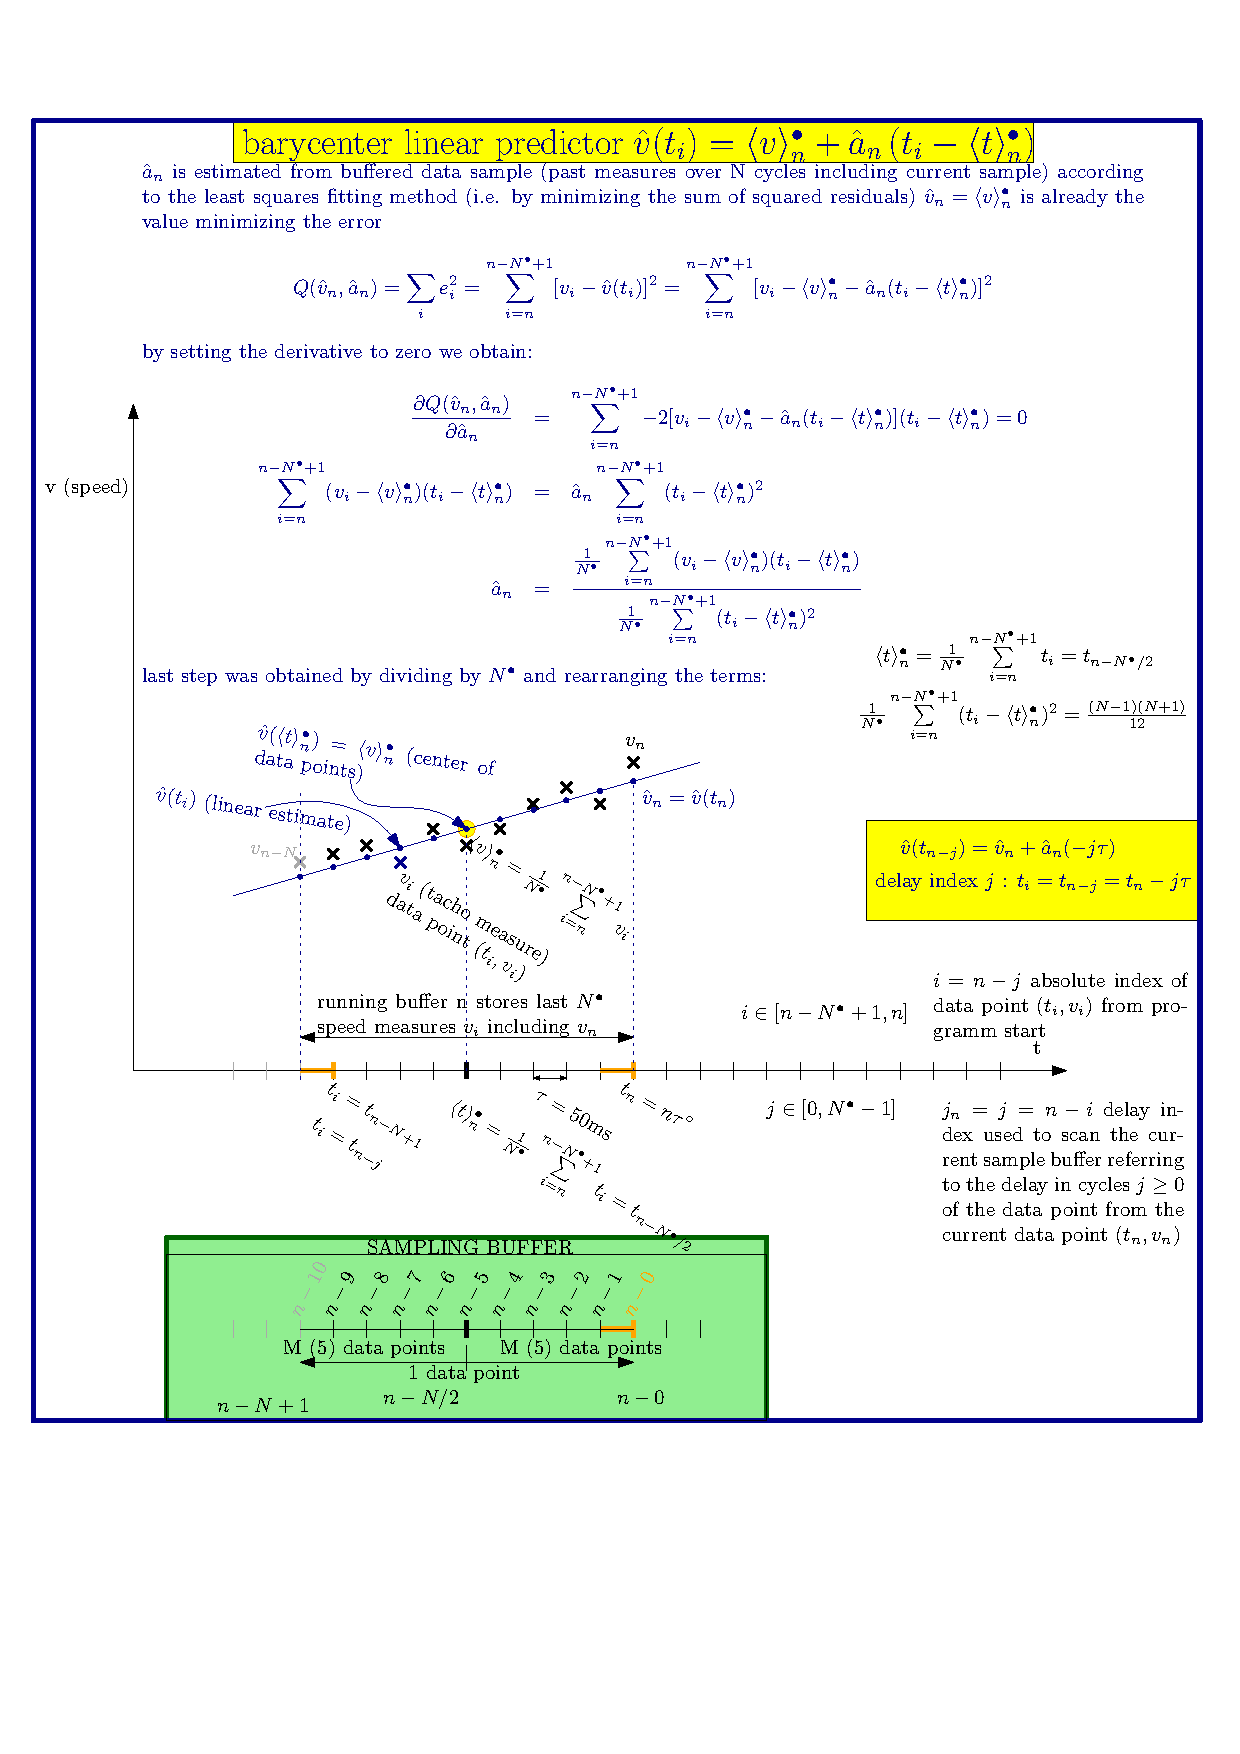
\includegraphics[angle=-0,width=1.\textwidth]{lin_can_regression_v2.pdf}
	}
	\caption{\emph{estimate acceleration applying linear regression}}
	\label {fig:lcregression}
\end{figure}

\noindent
%%%%%%%%%%%%%%%
%%% INPUT:
\begin{minipage}[t]{8ex}{\color{red}\bf
		\begin{verbatim}
		(%i22) 
		\end{verbatim}
	}
\end{minipage}
\begin{minipage}[t]{\textwidth}{\color{blue}
		\begin{verbatim}
		load("simplify_sum");
		sum(j^2,j,0,N);
		simplify_sum(%);
		\end{verbatim}
	}
\end{minipage}


%%% OUTPUT:
\definecolor{labelcolor}{RGB}{100,0,0}
\begin{math}\displaystyle
	\parbox{8ex}{\color{labelcolor}(\%o22) }
	/usr/share/maxima/5.32.1/share/solve\_rec/simplify\_sum.mac
\end{math}

\begin{math}\displaystyle
	\parbox{8ex}{\color{labelcolor}(\%o23) }
	\sum_{j=0}^{N}{j}^{2}
\end{math}

\begin{math}\displaystyle
	\parbox{8ex}{\color{labelcolor}(\%o24) }
	\frac{2\,{N}^{3}+3\,{N}^{2}+N}{6}
\end{math}
%%%%%%%%%%%%%%%

\noindent
%%%%%%%%%%%%%%%
%%% INPUT:
\begin{minipage}[t]{8ex}{\color{red}\bf
		\begin{verbatim}
		(%i1) 
		\end{verbatim}
	}
\end{minipage}
\begin{minipage}[t]{\textwidth}{\color{blue}
		\begin{verbatim}
		load("simplify_sum");
		(1/(N+1))*sum(((N)/2-j)^2,j,0,N);
		expand(simplify_sum(%));
		\end{verbatim}
	}
\end{minipage}

%%% OUTPUT:
\definecolor{labelcolor}{RGB}{100,0,0}
\begin{math}\displaystyle
	\parbox{8ex}{\color{labelcolor}(\%o1) }
	/usr/share/maxima/5.32.1/share/solve\_rec/simplify\_sum.mac
\end{math}

\begin{math}\displaystyle
	\parbox{8ex}{\color{labelcolor}(\%o2) }
	\frac{\sum\limits_{j=0}^{N}{\left( \frac{N}{2}−j\right) }^{2}}{N+1}
\end{math}

\begin{math}\displaystyle
	\boxed{
		\parbox{8ex}{\color{labelcolor}(\%o3) }
		\frac{{N}^{3}}{12\,N+12}+\frac{2\,N}{12\,N+12}+\frac{{N}^{2}}{4\,N+4}
	}
\end{math}
%%%%%%%%%%%%%%%


\noindent
%%%%%%%%%%%%%%%
%%% INPUT:
\begin{minipage}[t]{8ex}{\color{red}\bf
		\begin{verbatim}
		(%i4) 
		\end{verbatim}
	}
\end{minipage}
\begin{minipage}[t]{\textwidth}{\color{blue}
		\begin{verbatim}
		ratsimp(%);
		\end{verbatim}
	}
\end{minipage}
%%% OUTPUT:
\definecolor{labelcolor}{RGB}{100,0,0}
\begin{math}\displaystyle
	\boxed{
		\parbox{8ex}{\color{labelcolor}(\%o4) }
		\frac{{N}^{2}+2\,N}{12}
	}
\end{math}
%%%%%%%%%%%%%%%

\noindent
%%%%%%%%%%%%%%%
%%% INPUT:
\begin{minipage}[t]{8ex}{\color{red}\bf
		\begin{verbatim}
		(%i9) 
		\end{verbatim}
	}
\end{minipage}
\begin{minipage}[t]{\textwidth}{\color{blue}
		\begin{verbatim}
		load("simplify_sum");
		(1/(N+1))*sum(((N)/2-j),j,0,N);
		expand(simplify_sum(%));
		ratsimp(%);
		\end{verbatim}
	}
\end{minipage}
%%% OUTPUT:
\definecolor{labelcolor}{RGB}{100,0,0}
\begin{math}\displaystyle
	\parbox{8ex}{\color{labelcolor}(\%o9) }
	/usr/share/maxima/5.32.1/share/solve\_rec/simplify\_sum.mac
\end{math}

\begin{math}\displaystyle
	\boxed{
		\parbox{8ex}{\color{labelcolor}(\%o10) }
		\frac{1}{N+1}\sum\limits_{j=0}^{N}\left(\frac{N}{2}−j\right)=0
	}
\end{math}

%%%%%%%%%%%%%%%
\newpage

================================


following extract is obtained by using \emph{copy latex} from Maxima (examples intended to help to evaluate the expressions above)
\begin{figure}
	\centerline{
		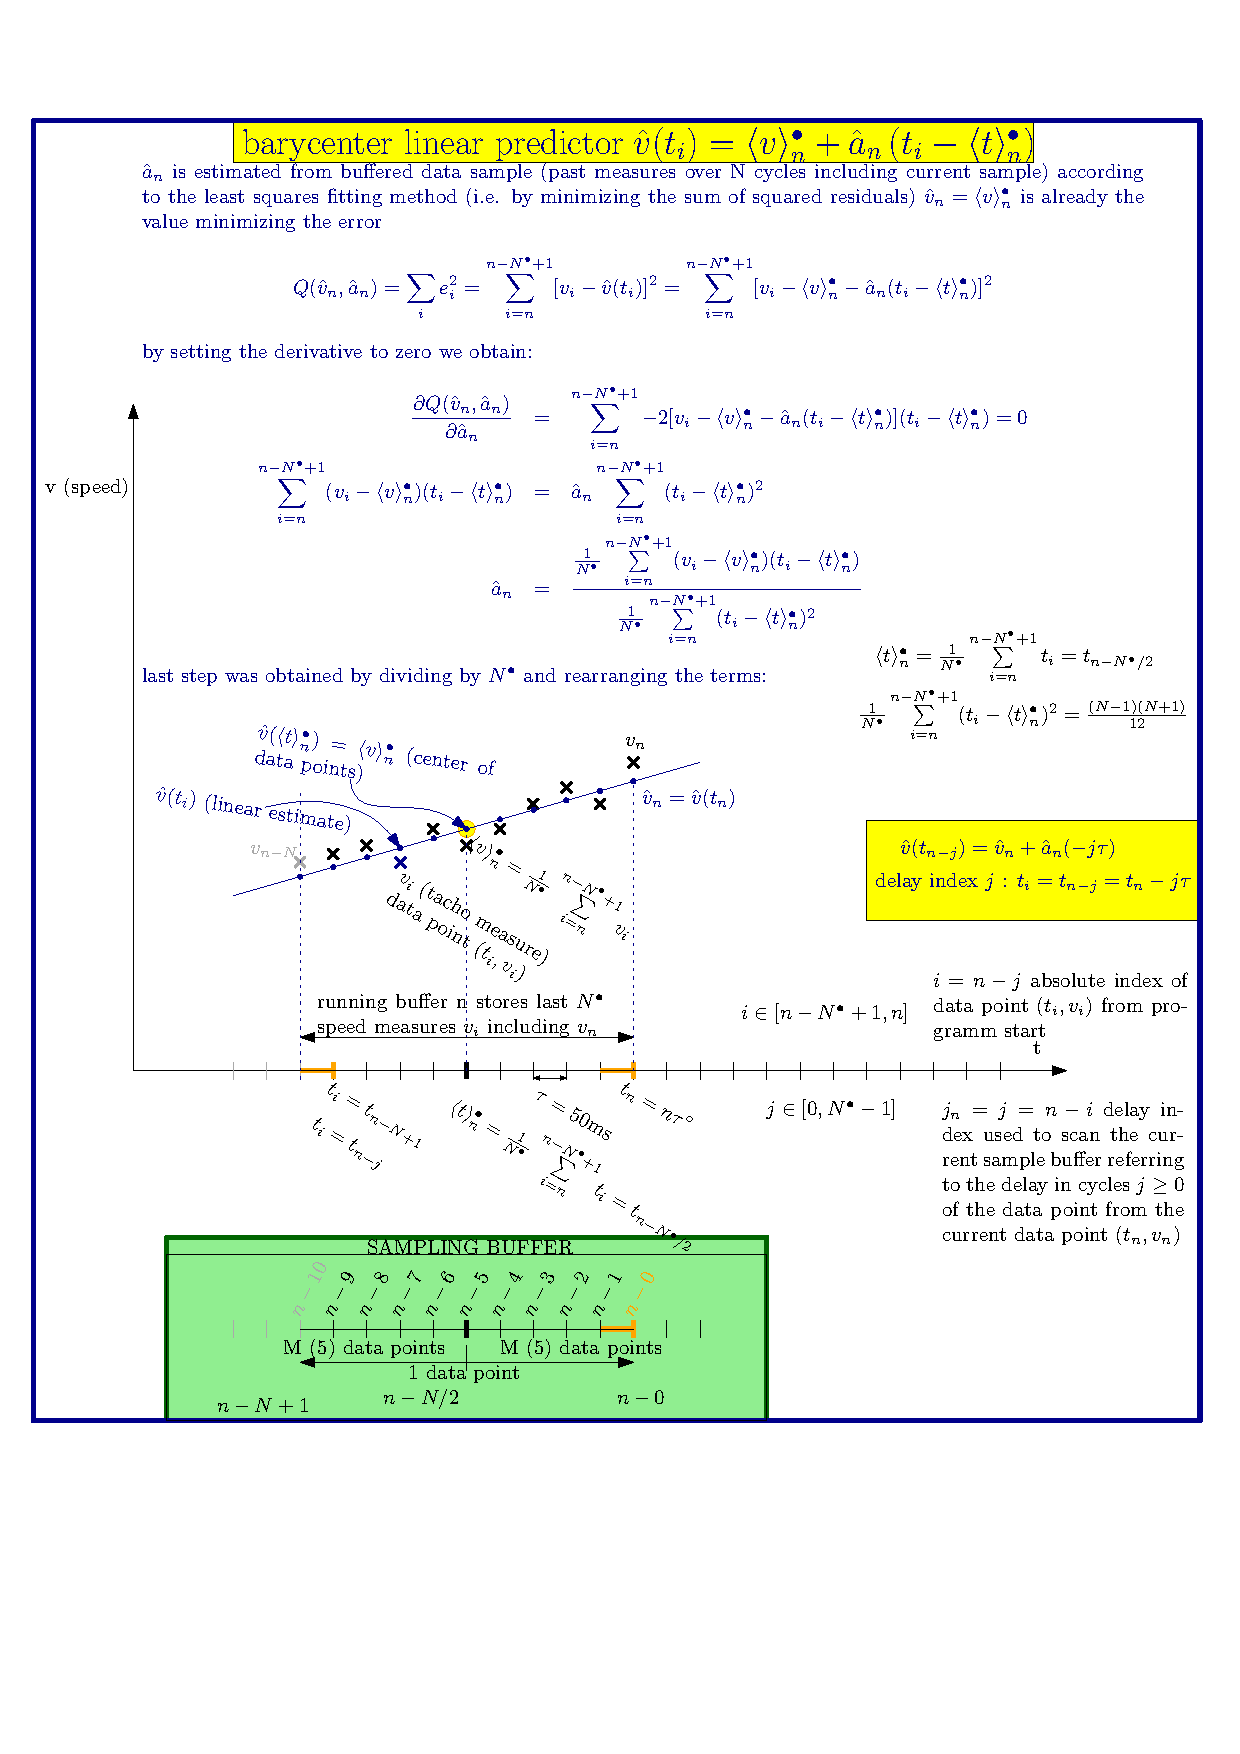
\includegraphics[angle=-0,width=1.\textwidth]{lin_can_regression_v2.pdf}
	}
	\caption{\emph{estimate acceleration applying linear regression}}
	\label {fig:lcregression}
\end{figure}

\noindent
%%%%%%%%%%%%%%%
%%% INPUT:
\begin{minipage}[t]{8ex}{\color{red}\bf
		\begin{verbatim}
		(%i22) 
		\end{verbatim}
	}
\end{minipage}
\begin{minipage}[t]{\textwidth}{\color{blue}
		\begin{verbatim}
		load("simplify_sum");
		sum(j^2,j,0,N);
		simplify_sum(%);
		\end{verbatim}
	}
\end{minipage}


%%% OUTPUT:
\definecolor{labelcolor}{RGB}{100,0,0}
\begin{math}\displaystyle
	\parbox{8ex}{\color{labelcolor}(\%o22) }
	/usr/share/maxima/5.32.1/share/solve\_rec/simplify\_sum.mac
\end{math}

\begin{math}\displaystyle
	\parbox{8ex}{\color{labelcolor}(\%o23) }
	\sum_{j=0}^{N}{j}^{2}
\end{math}

\begin{math}\displaystyle
	\parbox{8ex}{\color{labelcolor}(\%o24) }
	\frac{2\,{N}^{3}+3\,{N}^{2}+N}{6}
\end{math}
%%%%%%%%%%%%%%%

\noindent
%%%%%%%%%%%%%%%
%%% INPUT:
\begin{minipage}[t]{8ex}{\color{red}\bf
		\begin{verbatim}
		(%i1) 
		\end{verbatim}
	}
\end{minipage}
\begin{minipage}[t]{\textwidth}{\color{blue}
		\begin{verbatim}
		load("simplify_sum");
		(1/(N+1))*sum(((N)/2-j)^2,j,0,N);
		expand(simplify_sum(%));
		\end{verbatim}
	}
\end{minipage}

%%% OUTPUT:
\definecolor{labelcolor}{RGB}{100,0,0}
\begin{math}\displaystyle
	\parbox{8ex}{\color{labelcolor}(\%o1) }
	/usr/share/maxima/5.32.1/share/solve\_rec/simplify\_sum.mac
\end{math}

\begin{math}\displaystyle
	\parbox{8ex}{\color{labelcolor}(\%o2) }
	\frac{\sum\limits_{j=0}^{N}{\left( \frac{N}{2}−j\right) }^{2}}{N+1}
\end{math}

\begin{math}\displaystyle
	\boxed{
		\parbox{8ex}{\color{labelcolor}(\%o3) }
		\frac{{N}^{3}}{12\,N+12}+\frac{2\,N}{12\,N+12}+\frac{{N}^{2}}{4\,N+4}
	}
\end{math}
%%%%%%%%%%%%%%%


\noindent
%%%%%%%%%%%%%%%
%%% INPUT:
\begin{minipage}[t]{8ex}{\color{red}\bf
		\begin{verbatim}
		(%i4) 
		\end{verbatim}
	}
\end{minipage}
\begin{minipage}[t]{\textwidth}{\color{blue}
		\begin{verbatim}
		ratsimp(%);
		\end{verbatim}
	}
\end{minipage}
%%% OUTPUT:
\definecolor{labelcolor}{RGB}{100,0,0}
\begin{math}\displaystyle
	\boxed{
		\parbox{8ex}{\color{labelcolor}(\%o4) }
		\frac{{N}^{2}+2\,N}{12}
	}
\end{math}
%%%%%%%%%%%%%%%

\noindent
%%%%%%%%%%%%%%%
%%% INPUT:
\begin{minipage}[t]{8ex}{\color{red}\bf
		\begin{verbatim}
		(%i9) 
		\end{verbatim}
	}
\end{minipage}
\begin{minipage}[t]{\textwidth}{\color{blue}
		\begin{verbatim}
		load("simplify_sum");
		(1/(N+1))*sum(((N)/2-j),j,0,N);
		expand(simplify_sum(%));
		ratsimp(%);
		\end{verbatim}
	}
\end{minipage}
%%% OUTPUT:
\definecolor{labelcolor}{RGB}{100,0,0}
\begin{math}\displaystyle
	\parbox{8ex}{\color{labelcolor}(\%o9) }
	/usr/share/maxima/5.32.1/share/solve\_rec/simplify\_sum.mac
\end{math}

\begin{math}\displaystyle
	\boxed{
		\parbox{8ex}{\color{labelcolor}(\%o10) }
		\frac{1}{N+1}\sum\limits_{j=0}^{N}\left(\frac{N}{2}−j\right)=0
	}
\end{math}

%%%%%%%%%%%%%%%
\newpage

================================

 MTBF of MMU subsystem & $>$ 30 000 hours \\
 \hline
 MTBF of each MMU board & $>$ 85 000 hours \\
 \hline

